\namedsection{Machine Learning}{Playle}
\label{ml}

%%%%%%%%%%%%%%%%%%%%%%%%%%%%%%%%% * Rewritten
%%% WHAT IS MACHINE LEARNING? %%%
%%%%%%%%%%%%%%%%%%%%%%%%%%%%%%%%%
Machine learning is a technique that takes some observations about a system in addition to some desired outputs, building a model around these parameters and uses this model to create predictions about the output for other observed data. There are typically three categories of machine learning algorithm: classification, where the output is in a finite set of classes; regression, where the output is continuous; and clustering, where the output of the algorithm are the groupings of observed data. In order to detect exercise, a supervised classifying machine learning algorithm will be most suitable, with the classes being types of activity observed.

\subsection{Considered Issues}

%%%%%%%%%%%%%%%%%%%%%%%%%%%%%%% * Okay
%%% CURSE OF DIMENSIONALITY %%%
%%%%%%%%%%%%%%%%%%%%%%%%%%%%%%%
One of the frequently encountered problems is the curse of dimensionality \cite{bellman1957dynamic}, whereby having a high number of dimensions, often as a result of having a large number of inputs into a machine learning algorithm, can create the problem where the amount of instances required to sufficiently train the model increases as the amount of training of the model must have instances such that the input feature space must be explored sufficiently \cite{oommen2008objective}. Further to this effect, the time and space complexity of many machine learning algorithms are functions of the feature space's dimensionality. However, existing work has demonstrated that the curse of dimensionality is not necessarily applicable to time-series data as the nature of such data explores the feature space on the condition that the signal-to-noise ratio is sufficiently high \cite{bernecker2011quality}.

%%%%%%%%%%%%%%%%%%% * Okay
%%% OVERFITTING %%%
%%%%%%%%%%%%%%%%%%%
% Could do with some cites, but I can't find any decent ones
Another problem encountered in machine learning is that of overfitting, where the model for some algorithm is trained such that it specialises on the training set alone. This can be problematic where the model is introduced to new data, as such models have poor performance on unseen data. Overfitting can be prevented by reducing the complexity of the model, as if the model is not complex enough, it is not possible for it to overfit on the training data exactly. Additionally, testing should be performed on a data set other than the training set, which can be achieved with using some form of cross-validation, or even having a completely separate data set on which to test.

\subsection{Initial Feasibility Assessment}
%%%%%%%%%%%%%%%%%%%% * Okay 
%%% INTRO TO IFA %%%
%%%%%%%%%%%%%%%%%%%%
In order to initially determine the feasibility of applying machine learning for detecting exercise, a simple experiment was conducted with a single subject. The intent of the experiment was to implement a similar machine learning algorithm as is described in \cite{kwapisz2011activity} to ensure understanding of the problem at hand and identify any issues with such a set-up.

%%%%%%%%%%%%%%%%%%%%%%%%%%%%%% * Okay
%%% IFA EXPERIMENTAL SETUP %%%
%%%%%%%%%%%%%%%%%%%%%%%%%%%%%%
% Maybe reword "random", doesn't sound right
The collection device used came in the form of a Sony Z3 mobile phone, providing kinematic sensors, of which the gyroscope, measuring the angular velocity was used. The subject had the collection device attached to their foot while they performed activities including a foot rotation exercise; walking on a flat surface; and walking up and down stairs. Additionally, noise was collected by moving the collection device in random directions. The collection device sampled data at 200Hz on each axis, so for the purpose of assessing feasibility, this value was carried through into machine learning, using a window size of 200 samples for a classification over 1 second intervals. In this machine learning technique, the window of samples is treated as a single instance of data to be classified. Each new classification will therefore shift the window forwards by a single time step to produce a new instance.

%%%%%%%%%%%%%%%%%%%%%%%%% * Okay
%%% MORE ON IFA SETUP %%%
%%%%%%%%%%%%%%%%%%%%%%%%%
% Could further this
Data for each activity was collected separately to ensure classification could be performed without having to note exact timings of activities. Some examples of the data collected in these activities are shown in figure \ref{fig:first-data}, where the periodic nature of all the activities (with the exception of noise), can be seen clearly.

%%%%%%%%%%%%%%%%%%% * Okay
%%% IFA RESULTS %%%
%%%%%%%%%%%%%%%%%%%
This data was run through a series of tools to build a model, as described in section \ref{sec:tools-produced}. Initial evaluation of the performance was conducted using 10-fold cross-validation with the confusion matrix for a simple naive Bayes classifier shown in table \ref{tab:first-confusion}, giving a classification accuracy of 89\%. Despite the data only being collected from a single individual using a small set of instances, the results were considered promising, indicating that this machine learning technique as a method of activity recognition was feasible.

\begin{table}
	\centering
	\begin{tabular}{|cccc|ll|}
		\hline
		\multicolumn{4}{|c|}{Classified As}   &          &                        \\
		Exercise & Noise & Stairs & Walking &          &                        \\
		\hline
		62       & 0     & 0      & 0       & Exercise & \multirow{4}{*}{Class} \\
		2        & 15    & 1      & 0       & Noise    &                        \\
		3        & 0     & 10     & 3       & Stairs   &                        \\
		1        & 0     & 1      & 7       & Walking  &                       \\
		\hline
	\end{tabular}
	\caption{Feasibility assessment confusion matrix \label{tab:first-confusion}}
\end{table}

% Axes labels!
\begin{figure}
	\centering
	\subfigure[Exercise]{\label{fig:first-exercise}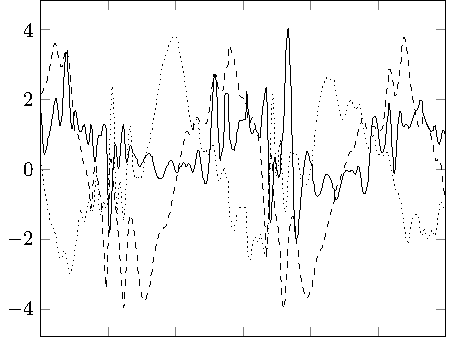
\includegraphics[width=70mm]{figures/first-exercise.pdf}}
	\subfigure[Noise]{\label{fig:first-noise}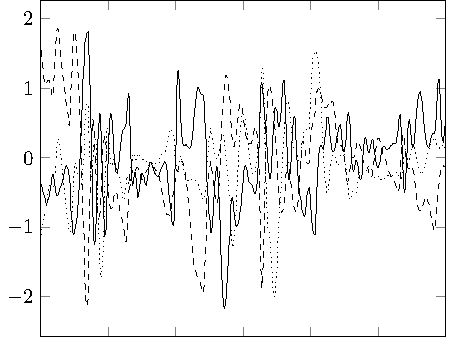
\includegraphics[width=70mm]{figures/first-noise.pdf}}
	\subfigure[Stairs]{\label{fig:first-stairs}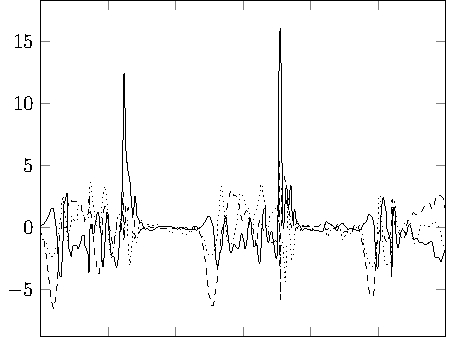
\includegraphics[width=70mm]{figures/first-stairs.pdf}}
	\subfigure[Walking]{\label{fig:first-walking}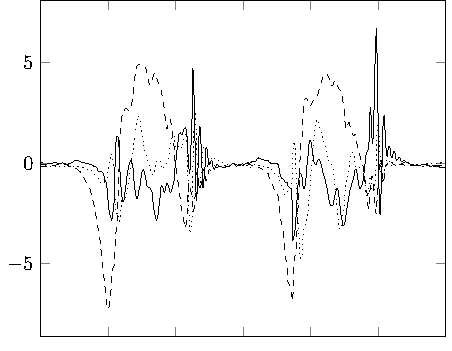
\includegraphics[width=70mm]{figures/first-walking.pdf}}
	\caption{Feasibility assessment of collected data \label{fig:first-data}}
\end{figure}


\subsection{Tools \label{sec:tools}}
%%%%%%%%%%%%%%%%%%%%%%%%%%%%% * Okay
%%% TOOLS USED / PRODUCED %%%
%%%%%%%%%%%%%%%%%%%%%%%%%%%%%
% Could perhaps do with more content
Weka, a machine learning library, was used extensively for machine learning aspects. It provides a vast multitude of implemented machine learning algorithms, including various methods of evaluating the performance of these trained models.

%%%%%%%%%%%%%%%%%%%%%%% * Okay
%%% THE ARFF SCRIPT %%%
%%%%%%%%%%%%%%%%%%%%%%%
Weka accepts instances in the form of an \texttt{.arff} file, this file specifies all the classes for the classifier to accept; the inputs for the classifier; and some number of instances and their actual class, if known. In order to produce this, it is first necessary to know the desired classification over given intervals for some time series data. This is achieved by mapping a single point of interest on some time series data to a class. This mapping, along with the number of samples for each window is then passed to a script that makes windows centered on these points of interest and creates the corresponding \texttt{.arff}.

%%%%%%%%%%%%%%%%%%%% * Okay
%%% DOWNSAMPLING %%%
%%%%%%%%%%%%%%%%%%%%
Data collection is already an expensive task in terms of time consumed. It was therefore deemed infeasible to sample at multiple frequencies on top of all the variables being explored during data collection. Further to this, the device being used for data collection was not flexible enough in terms of allowable sampling frequencies. To allow for analysis of multiple sampling frequencies at a later data, sampling was done at 200Hz, the fastest the collection device would allow. Any collected data could then be downsampled, which was achieved by taking the closest sample to $n/f$ where f is the frequency to downsample to.

%%%%%%%%%%%%%%%%%%%%%% * Okay
%%% CLASSIFICATION %%%
%%%%%%%%%%%%%%%%%%%%%%
As shown in figure \ref{fig:first-data}, activities of interest produce periodic data in a way that the key features of a given activity can be considered trivial to identify should the activity be known to the manual classifier. This characteristic of the collected data was used to identify the ideal intervals for classification. Collected data was separated at the time of collection into individual files each representing a different activity/sensor tuple, allowing for manual classification. 

%%%%%%%%%%%%%%%%%%%%%%%%%%%%%%%%%%%%%%%% * Okay
%%% HOW CLASSIFICATION WAS PERFORMED %%%
%%%%%%%%%%%%%%%%%%%%%%%%%%%%%%%%%%%%%%%%
The act of data classification occurred by viewing the plotted data from which the points of interest were noted. For the \textit{not exercise} class, points of interest were taken at frequent points throughout collected data files where subjects were not performing exercise, meaning that manual classification of the \textit{not exercise} class was not required. These points of interest are then ready to be passed to the script to generate the \texttt{.arff} file.

\subsection{Evaluating Performance}
%%%%%%%%%%%%%%%%%%%%%%%%%%%%%%%%%%%%%%%%%%%%%%%%%%%%%%%%%
%%% ASSESSING MODEL PERFORMANCE - WHY ACCURACY IS BAD %%%
%%%%%%%%%%%%%%%%%%%%%%%%%%%%%%%%%%%%%%%%%%%%%%%%%%%%%%%%%
There are multiple methods of assessing the performance of a model. A simple assessment may include measuring the accuracy, that is, just looking at the number of correctly and incorrectly classified instances, although this does not take into account the probability of specific classes existing, and can therefore skew results when there are significantly more instances of a subset of classes over another subset of classes. An extreme example of this is the 0-R classifier, which will determine the modal class of some training set and classify all instances as this. Such a classifier is very simple, and has a severely limited utility, but depending on the distribution of instanced between classes, a high accuracy may be possible, despite what can be considered poor classifying behaviour.

%%%%%%%%%%%%%%%%%%%%%%%%%%% * Okay
%%% THE KAPPA STATISTIC %%%
%%%%%%%%%%%%%%%%%%%%%%%%%%%
By taking into account the probability of instances being in any given class, the bias that leads to this poor metric can be eliminated. Such a statistic is the kappa statistic, which measures performance with respect to a null classifier, that is, a classifier that solely takes into account the frequencies of observed data \cite{viera2005understanding}. A kappa statistic, $\kappa < 0$  would indicate very bad performance (worse than guessing while only taking into account the class frequencies). $\kappa > 0$ indicates better performance, with $\kappa = 1$ being a perfect classifier. The kappa statistic has therefore been used to measure the performance of later classifiers.

%%%%%%%%%%%%%%%%%%%%%%%%%%%%%
%%% CUSTOM COST FUNCTIONS %%%
%%%%%%%%%%%%%%%%%%%%%%%%%%%%%
% I don't like this paragraph
In some cases, it may be important to quantify the trade-off a classifier makes between true and false positives. This can especially be the case where it is more important to detect some class over another. Achieving this can be done with a cost function, which is applied to the resultant confusion matrix (equation \ref{eq:cost}). From this, the average cost per instance can be computed, allowing comparisons to be drawn. This method of performance evaluation is similar to an ROC curve, except where an ROC curve shows performance with varying discriminating thresholds, cost functions dictate where the threshold must lie.

\begin{equation}
	\label{eq:cost}
	\begin{gathered}
		\text{Cost } c = \langle \mathbf{COST}, \mathbf{CONFUSION} \rangle_F \\
		\text{Where $\langle \mathbf{A}, \mathbf{B}\rangle_F$ is the Frobenius inner product between $\mathbf{A}$ and $\mathbf{B}$}
	\end{gathered}
\end{equation}

\subsection{Considered Algorithms}
% This could do with an introduction, although I can't think of anything meaningful to put here

\subsubsection{Multilayer Perceptrons}
%%%%%%%%%%% * Okay
%%% MLP %%%
%%%%%%%%%%%
A Multilayer Perceptron (MLP) is a type of Neural Network where the nodes, or perceptrons, are organised in layers. Each node accepts some number of inputs with some weight, and the summation of these weighted inputs are computed and applied to some activation function, the result of which is the output of the node (equation \ref{eq:perceptron}).

\begin{equation}
\label{eq:perceptron}
\text{Output } o = activation\bigg(\sum_{i=1}^{d}{x_iw_i}\bigg) 
\end{equation}

%%%%%%%%%%%%% * Not too bad
%%% MLP 2 %%%
%%%%%%%%%%%%%
Each perceptron effectively defines a plane in $d$-dimensional space. Instances on either side of this plane can then be classed, allowing a single perceptron to act as a simple classifier. By combining multiple perceptrons in a layer, it is possible to build up these planes in order to create more complex classifier made of these linear classifiers. The addition of layers, using previous layers as inputs allows a more complex classifier still by allowing the importance of these sub-classifiers to vary with the inputs. MLPs with enough inputs and layers can therefore replicate any function \cite{baum1988capabilities}.

\begin{figure}
	\centering
	% I'm not too happy with this, but it'll do, I guess...
	% Might get rid of this actually...
	\begin{tikzpicture}[shorten >=1pt,node distance=1.3cm and 3cm,on grid,auto,initial text={}] 
	\node[state,rectangle] (i1) {$i_1$};
	\node[state,rectangle] (i2) [below=of i1] {$i_2$}; 
	\node[state,rectangle] (in) [below=of i2] {$i_n$}; 
	
	\node[state] (h11) [right=of i1] {$h_{1,1}$};
	\node[state] (h12) [below=of h11] {$h_{1,2}$}; 
	\node[state] (h1a) [below=of h12] {$h_{1,a}$}; 
	
	\node[state] (hb1) [right=of h11] {$h_{b,1}$};
	\node[state] (hb2) [below=of hb1] {$h_{b,2}$}; 
	\node[state] (hba) [below=of hb2] {$h_{b,a}$}; 
	
	\node[state] (o) [right=of hb2] {$o$};
	\path[->] 
	(i1) edge node {} (h11) (i2) edge node {} (h11)
	(i1) edge node {} (h12) (i2) edge node {} (h12)
	(i1) edge node {} (h1a) (i2) edge node {} (h1a)
	(in) edge node {} (h11) (h11) edge node {} (hb1)
	(in) edge node {} (h12) (h11) edge node {} (hb2)
	(in) edge node {} (h1a) (h11) edge node {} (hba)
	(h12) edge node {} (hb1) (h1a) edge node {} (hb1)
	(h12) edge node {} (hb2) (h1a) edge node {} (hb2)
	(h12) edge node {} (hba) (h1a) edge node {} (hba)
	
	(hb1) edge node {} (o)
	(hb2) edge node {} (o)
	(hba) edge node {} (o)
	;
	\end{tikzpicture}
	\caption{Example topology of a MLP \label{fig:mlp-topology}}
\end{figure}

\subsubsection{Radial Basis Function Networks}
%%%%%%%%%%% * Okay
%%% RBF %%%
%%%%%%%%%%%
A Radial Basis Function (RBF) network is a type of Neural Network that is composed of 2 layers, an input layer and an output layer. The activation functions for this output layer are RBFs, where an RBF can be any function that is only dependent on the distance from some point. An example of a commonly used RBF is the Gaussian function. RBF networks are quite similar to MLPs, with the main difference being hidden layers and the activation function \cite{broomhead1988radial}.

%%%%%%%%%%%%%%%%%%%%%%%%%%%%%%%%%%%%%% * Okay
%%% WHY RBF IS BAD FOR CONSTRAINED %%%
%%%%%%%%%%%%%%%%%%%%%%%%%%%%%%%%%%%%%%
For the RBF network, as a Gaussian function is typically used, this can be troublesome for constrained systems, as the need to compute the probability density function for each RBF can require significant resources. Equation \ref{eq:mvg} shows the formula for computing the probability density function for a multivariate Gaussian distribution, which for a large number of inputs to the machine learning algorithm will result in having to perform matrix operations in large dimensions. An approximation of this formula can be made, but an implementation on a constrained device would prove challenging, as the approximation results in a higher memory usage.

\begin{equation}
	pdf(\mathbf{x}) = (2\pi)^{-\frac{k}{2}}|\mathbf{\Sigma}^{-\frac{1}{2}}|e^{-\frac{1}{2}(\mathbf{x}-\mathbf{\mu})'\mathbf{\Sigma^{-1}}(\mathbf{x}-\mathbf{\mu})}
	\label{eq:mvg}
\end{equation}

\subsubsection{Instance-Based Learning}
%%%%%%%%%%%%%%%%%%% *Okay
%%% IBL GENERAL %%%
%%%%%%%%%%%%%%%%%%%
Instance-based learning is a type of machine learning algorithm that postpones model creation until an output for a problem instance is required. Some number of labelled instances are stored in memory, and these are used to label problem instances.

%%%%%%%%%%%%%%%%%% *Okay
%%% IBL UPDATE %%%
%%%%%%%%%%%%%%%%%%
Instance-based learning is advantageous over other machine learning methods in that adapting the model with new instances is trivial. This makes it attractive for simple systems where some adaptation of the model is required.

%%%%%%%%%%%%%%%%%%%%%%%%%% *Okay
%%% IBL LOTS OF MEMORY %%%
%%%%%%%%%%%%%%%%%%%%%%%%%%
As a number of labelled instances must be kept in memory in order to compute the model, instance-based learning methods can require large amounts of memory to classify. Additionally, any problem instances must be compared against each labelled instance that is to be used for the model, meaning that time complexity for classification of any problem instance is linear in the number of labelled instances. This can present significant challenges when the size of the training data set become large with respect to the underlying device.

%%%%%%%%%%% *Okay
%%% kNN %%%
%%%%%%%%%%%
An example of instance-based learning is the k-nearest neighbours algorithm, where any problem instance is compared to the k-nearest labelled instances. The majority class of these nearest instances would be used as the class for the problem instance.

\subsubsection{Trade-offs and Parameters}

%%%%%%%%%%%%%%%%%%%%%%%%%%%%
%%% ALGORITHM PARAMETERS %%%
%%%%%%%%%%%%%%%%%%%%%%%%%%%%
There are many parameters that affect the performance of classifiers. In the case of the collected data, the sampling frequency for the kinematic sensor and the window with a number of samples over which the classifier classifies have a direct impact on the classifier's ability to perform. In the case of the model, most machine learning algorithms have some form parameters allowing their behaviour to change. 

\begin{figure}
	\centering
	\subfigure[Top-Down]{\label{fig:mlp-multi-flat}\includegraphics[width=70mm]{figures/mlp-multi-analysis-flat.pdf}}
	\subfigure[Side-On, Varying Hidden Layers]{\label{fig:mlp-multi-3d}\includegraphics[width=64mm]{figures/mlp-multi-analysis-3d.pdf}}
	%\subfigure[Varying Frequency]{\label{fig:mlp-multi-3d-2}\includegraphics[width=70mm]{figures/mlp-multi-analysis-3d-2.pdf}}
	\subfigure[3D Surface Plot]{\label{fig:mlp-multi-3d-3}\includegraphics[width=90mm]{figures/mlp-multi-analysis-3d-3.pdf}}
	\caption{MLP Parameter Performance Surface Plot \label{fig:mlp-multi}}
\end{figure}

%%%%%%%%%%%%%%%%%% * Okay, maybe reword
%%% MLP PARAMS %%%
%%%%%%%%%%%%%%%%%%
For the MLP, the number of hidden layers is the most important parameter, so analysis on this and the sampling frequency was performed, as shown in figure \ref{fig:mlp-multi}, where the performance is plotted as a function of both of these parameters. Figure \ref{fig:mlp-multi-flat} shows that above 6 hidden layers while sampling at around 20Hz, performance roughly levels out. An interesting observation can be made in figure \ref{fig:mlp-multi-3d}, where the performance for 1 hidden layer was significantly worse than 0 hidden layers.

%%%%%%%%%%%%%%%%%%%%%%%%%%%%% * Okay
%%% 3 CLASSES OVER JUST 2 %%%
%%%%%%%%%%%%%%%%%%%%%%%%%%%%%
% Maybe add transision figure
The number of classes to classify was considered as a variable parameter for the classifier. A classifier with the 2 classes \textit{activity} and \textit{not activity}, would only allow for binary classification. Depending on the classifier behaviour and the nature of the exercise in question, it may be the case that when the window of classification lies between 2 classes, such a window could be classified as either class. This unpredictable behaviour would prevent further analysis of the subject's activity beyond how much time a given activity was detected for. However, by splitting the \textit{activity} class into 2 distinct classes, such that every activity performed will always be composed of these parts, it allows 3 classes to be used with the classifier. Such a change would allow counting of distinct activities, by ensuring that one type of \textit{activity} class is followed by the other type of \textit{activity} class. This would allow the number of exercises to be counted, as well as the amount of time exercised. Further to this, the additional information this provides may allow for heuristics to increase accuracy should the classifier ``bounce'' during a transition between classes. Other numbers of classes were also considered, such as some number of classes for the exercise, along with a class for each likely type of non-exercise activity, however this was ultimately rejected due to the increased complexity of the system, leading to further resource consumption for the constrained system, while the performance of the algorithm was already considered satisfactory. For the final machine learning algorithm, the subclasses for the activity were based on the peaks and troughs of the y-axis data. This data was determined to be quite clear for manual classification.

%%%%%%%%%%%%%%%%%%%%%%%%%%
%%% USER STUDY RESULTS %%%
%%%%%%%%%%%%%%%%%%%%%%%%%%
\subsection{User Study Results}
%\note{As a result of the user study, how did the results change? Note observed results due to the user study.}
%The user study was performed on a number subjects, where both accelerometer and gyroscope data was collected for multiple activities.

\begin{figure}
	\includegraphics[width=\linewidth]{subject-fold-results.pdf}
	\caption{Subject Performance with Different Sensors and Algorithms \label{fig:subfold}}
\end{figure}

%%%%%%%%%%%%%%%%%%%%%%%%%%%%%%%%%%% * Okay
%%% WHY CROSS-VALIDATION IS BAD %%%
%%%%%%%%%%%%%%%%%%%%%%%%%%%%%%%%%%%
To evaluate the models on the user study data, cross-validation was considered, as this would allow training on some set of data and then testing on another set previously unseen to the model, although this would have the slightly undesirable effect of mixing data from subjects, whereas in practice, the device will be trained on a set of subjects and used by a subject not in that set. To replicate this kind of behaviour, a similar method to cross-validation was used, where the model was trained on all subjects, except for one. This one excluded subject was then tested on. This method is then repeated for all subjects. This subject-fold cross-validation method is also beneficial in allowing conclusions to be drawn about subject performance in relation to other subjects, assisting in determine which subjects should be used to produce the final model.

%%%%%%%%%%%%%%%%%%%%%%%%%%% * Okay
%%% SUBJECT PERFORMANCE %%% Woo, statistics!
%%%%%%%%%%%%%%%%%%%%%%%%%%%
Figure \ref{fig:subfold} shows the resultant performance, measured using the kappa statistic, for each of the subjects performing activities using different sensors sampling at 20Hz for the MLP and RBF classifiers. These results are collected using the subject-fold cross-validation technique as previously described. As the \textit{Accelerometer using MLP} result class was likely to require the most suitable for a low-power constrained device, this was used as a base-line to compare performance against. The null hypothesis was the mean of other result classes were equal to the mean of \textit{Accelerometer using MLP}. The alternative hypothesis was that these means were different. These hypotheses were tested using a series of \textit{t}-tests with significance level, $\alpha = 0.01$. The resultant $p$-values from these $t$-tests are displayed in table \ref{tab:res-ttest}. Despite the \textit{Gyroscope using MLP} and \textit{Accelerometer using RBF} result classes having a higher mean performance than \textit{Accelerometer using MLP} class, these increases were not statistically significant and therefore the null hypothesis in these cases could not be rejected. For \textit{Gyroscope using RBF}, a statistically significant change in mean performance was observed, leading to acceptance of the alternative hypothesis.

%%%%%%%%%%%%%%%%%%%%% * Okay
%%% MORE ANALYSIS %%%
%%%%%%%%%%%%%%%%%%%%%
Further analysis of the subject performance results show a large difference in performance between subjects. This can quite likely be attributed to some subjects performing the activities unlike the majority of other subjects, resulting in lower performance when they are used as the test data. In this result set, a single negative kappa statistic was observed, indicating that the performance was worse than guessing for this one case. However, generally, the performance for all result classes can be considered good.

\begin{table}
	\centering
	\begin{tabular}{l|ll}
		& Mean Performance & $p$-value \\
		\hline
		Accelerometer using MLP & 0.5842 & N/A \\
		Gyroscope using MLP     & 0.6204 & 0.6054 \\
		Accelerometer using RBF & 0.6116 & 0.5858 \\
		Gyroscope using RBF     & 0.8016 & $2.064 \times 10^{-4}$ \\        
	\end{tabular}
	\caption{Result classes statistical significance \label{tab:res-ttest}}
\end{table}

%%%%%%%%%%%%%%%%%%%%%%%%%%%%%%%%%%%%%%%%%%%%%% *Okay
%%% PERFORMANCE INCREASED WITH MORE PEOPLE %%%
%%%%%%%%%%%%%%%%%%%%%%%%%%%%%%%%%%%%%%%%%%%%%%
A noteworthy observation about the results was that after the first day of data collection, the performance of the model produced on this data was very poor. However, as the number of subjects increased after successive data collection days, so did the performance of the system. This would indicate that the algorithm was not able to fit properly on a small number of subjects, and that the introduction of more subjects was able to at least in part negate this.

%%%%%%%%%%%%%%%%%%%%%%%%%%% *Okay
%%% ALGORITHM SELECTION %%%
%%%%%%%%%%%%%%%%%%%%%%%%%%%
% Could cite that magic bullet paper here!
The main contenders for the algorithm were the MLP and RBF network due to high performance while having relatively low complexity, allowing them to be implemented without too much difficulty. Between these two algorithms, there was only a slight performance decrease in favour of the RBF network under some conditions, however, given the complexity of the RBF network's requirement for computing RBFs, this could create issues, especially given hardware constraints regarding a floating point number implementation. On the other hand, the MLP is very simple and approximations can be made such that only integers are required. For this reason, the MLP was selected to be used. As seen previously, 20Hz appeared to be the optimal sampling frequency, so this was selected to be used. The number of hidden layers is a trade-off between resources and performance, and it was decided that 2 hidden layers would provide sufficient performance while allowing for a reasonable demonstration of constrained machine learning.